\documentclass[11pt, a4paper]{article}
%\usepackage[danish]{babel}
\usepackage{amsmath}
\usepackage[utf8]{inputenc}
%\usepackage{xfrac}
\usepackage{amsfonts}
\usepackage{amssymb}
\usepackage{tikz}
\usepackage{array}
\usepackage{cancel}
\usepackage{ulem}
\usepackage{graphicx}
\usepackage[a4paper]{geometry}
\usepackage{gauss}
%\usepackage{mathtools}
\usepackage{amsmath}
\usepackage{lastpage}
\usepackage{fancyhdr}
\usepackage{multirow}
\usepackage{listings}
\setlength{\headheight}{15.2pt}
\pagestyle{fancy}
\fancyhf{}
\lhead{Mads Anthony, MANA} %husk denne
\rhead{Side\ \thepage\ af\ \pageref{LastPage}} %husk 2 builds for dette!
%\usepackage[ansinew]{inputenc} 
\usepackage{enumerate}
%dot2tex loads
\usetikzlibrary{shapes}
\begin{document}
\author{Mads Anthony}
\section{Methods}
In this section I will describe the methods that I've been using to evolve multitasking agents. Since most of these methods is build atop other methods, I've decided to start off with a description of the basics. I then use this as a foundation to describe the next methods that is building upon that. This bottom-up approach is then repeated until I've described all the methods used in this project.
\subsection{Evolutionary Algorithms}
Evolutionary Algorithms (EA) is a group of algorithms that are based on implementing the principles of evolution. The general idea is to mimic real life, and let the algorithm "discover" the best solutions. This is done by having a population of solutions be evaluated on a defined fitness parameter. We then let the fittest solutions survive, and combine them with another fit solution to produce a new offspring solution. The offspring then has a possibility to mutate and is placed in a new generation. We then repeat the procedure on the new generation until we have a good enough solution.
\\
\\
An overview of the algorithm can be seen in figure (x) and the following will give a more in-depth explanation of the components used to implement an EA.
\begin{figure}[!ht]
\centering
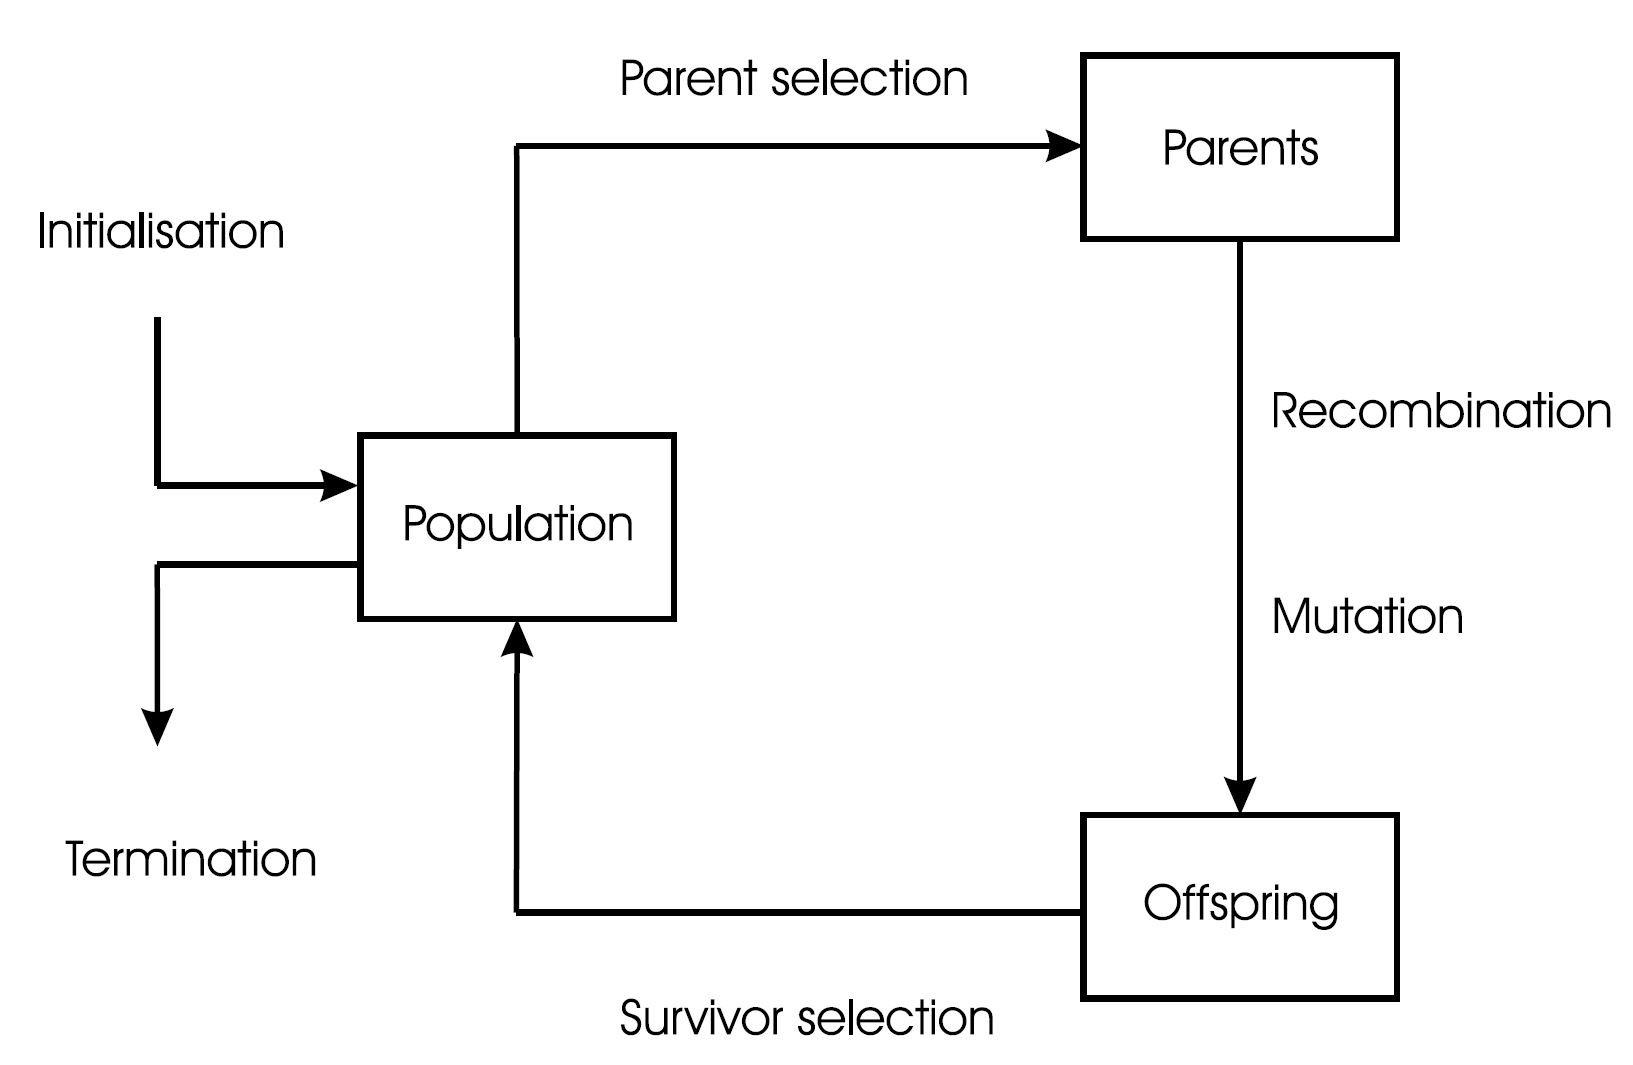
\includegraphics[scale=0.2]{EA_Figure}
\caption{[ref Eiben-Smith]}
\end{figure}
\subsubsection{Initialization}
To start using EA, we first need to have an initial population of individuals and decide how we want to represent these individuals. The representation of the individuals that the EA works with is called the genotype, and an individual that can be used on the actual problem domain is called the phenotype.
\\
\\
The phenotype space can be different from the genotype space, and choosing a genotype space is important, since it's here the evolutionary search takes place. The mapping from phenotype to genotype is called encoding and it is possible to have multiple genotypes that encode the same phenotype. The reverse is called decoding, however one genotype can only produce one phenotype.
\\
\\
With a representation chosen we can now initialise the first population. The initialisation of an EA is often kept simple, and the first population is therefore mostly generated randomly [p.23 Eiben Smith].
\subsubsection{Evaluation and Parent Selection}
With an initial population in place we now want to evaluate the whole population and choose which individuals will be used for parents. To do this, we introduce a fitness function. The fitness function is usually applied in the phenotype space (as it's here we want to find the best solution). The fitness of the genotype is therefore assigned by first decoding the genotype and then applying the fitness function.
\\
\\
Dependent on the problem being a minimisation or maximization problem we value the individuals with lowest or highest fitness values respectively. The idea for parent selection is to let the higher quality individuals be the base for the new generation. However we don't want to make the selection solely on the fitness, but instead use a probabilistic approach where individuals with higher fitness still gets favoured. This means that other  "weaker" individuals still get a chance to get picked. This is done to avoid the search being greedy and getting stuck on local optimum [p.21 Eiben-Smith].
\subsubsection{Recombination and Mutation}
Recombination merges two genotypes into one or more genotypes, and the way parts from the parents gets chosen, is decided in a randomly fashion. It is possible to use more than two parents but is not common as doesn't have a biological equivalent [p.22 Eiben-Smith]. Using only one parent is called a-sexual reproduction and can produce a different offspring dependent on the variation operator [ref?].
\\
\\
With a new offspring created there is a chance that a mutation might happen. A mutation will change the offspring's genotype in random unbiased way. This is done to fill the gene pool with "fresh blood" [p. 21 Eiben-Smith].
\subsubsection{Survivor Selection}
Survivor selection is similiar to parent selection, but is not stochastic. Instead it selects in a deterministic way by choosing from the unified multi set of parents and offspring the one with highest fitness.
\subsubsection{Termination}
When to terminate the EA can be chosen in many different ways. Some examples include: set a limit of number of generation or check if the diversity in the population drops under a certain a threshold.
\subsection{Neuroevolution}
Neuroevolution is evolutionary algorithms applied on artificial neural networks (ANN). In the following I will give an overview of what an ANN is and how they work.
\subsubsection{ANN}
ANN is a model that is inspired by biological neural networks - as observed in the brain. ANN is a collection of interconnected neurons and can be thought of as messages getting exchanged between each neuron. A single neuron can be defined in the following way.
\begin{figure}[!ht]
\centering
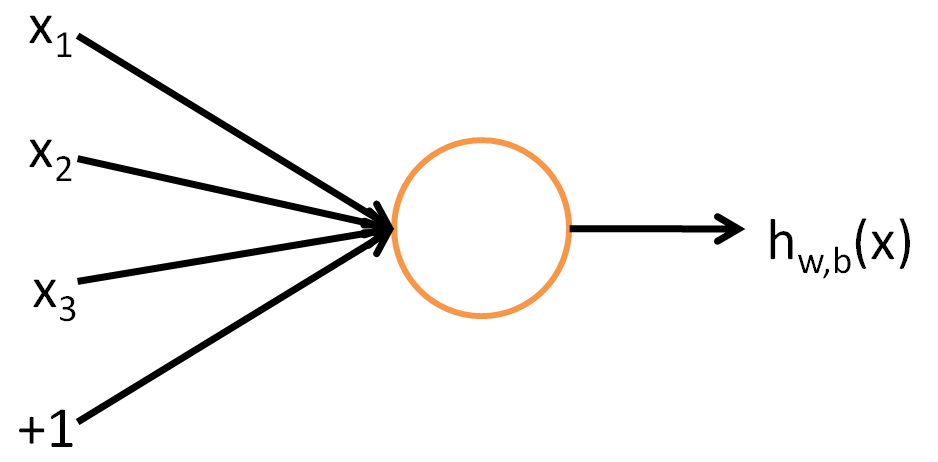
\includegraphics[scale=0.2]{SingleNeuron}
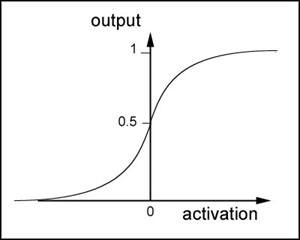
\includegraphics[scale=0.5]{sigmoid}
\caption{[ref http://ufldl.stanford.edu]}
\end{figure}
\\
As seen in figure (x), the neuron takes a number of inputs given by vector $ X $ and sums them together. It then inputs the sum into the the function $ h $ - also called an activation function. The idea with the activation function is... [ref].
\\
\\
The activation function can vary depending on the setup but often a sigmoid function is chosen. The one input to the neuron that is 1, is called a bias and can be grouped together with the vector $ X $ by setting $ X_0 = 1 $.
\\
\\
With the definition of a single neuron we can now connect them together with other neurons to get a larger network of neurons. However before we do that, we rewrite the input vector $ X $ as the product of a weight $ w $ and the output $ z $ of another neuron.
\begin{figure}[!ht]
\centering
\includegraphics[scale=0.7]{NeuralNetwork}
\caption{[ref - don't use this]}
\end{figure}
\\
\\
Each neuron can then be computed int the following.
\begin{equation}
z_k = h\Big(\sum\limits_{j}{w_{kj} z_j}\Big)
\end{equation}
ANN has three different types of layers as shown in figure (x). An input layer that takes the input often along with a bias. A hidden layer that connects the input layer to either the output or a new hidden layer. An output layer then uses the connections from the hidden (and input - if any connection) layer to produce the output. 
\\
\\
It's possible to have cyclic connections, ex. a neuron connected to itself, but the networks I train in this project is feed forward and don't have any cycles. 
\\
\\
Neural networks can also be used in standard classification task by feeding the network an input and compare the output with a target output using an error term. This error term can then be minimized by setting the weights using the back propagation algorithm. However in neuroevolution we don't set the weights using back propagation, but instead let an evolutionary algorithm decide.
\subsection{NEAT}
\subsection{HyperNEAT}
\subsection{Compositional Pattern Producing Network (CPPN)}
\subsection{Single Unit Pattern Generator (SUPG)}
\end{document}